\section{Free Scalar Field Theory Part 2, Lorentz Invariance}
Recall the action for a collection of QSHOs coupled with nearest neighbour interactions:
\begin{equation}
    S = \sum_{j=1}^M \int dt \frac{1}{2}\dot{\phi}_j^2 - \frac{1}{2}\omega_0^2\phi_j - \frac{1}{2}\frac{c^2}{\delta^2}\left(\phi_j - \phi_{j+1}\right)^2
\end{equation}
where we have periodic boundary conditions, such that $\phi_{j+M} = \phi_j$. The lattice spacing is $\delta$ such that the total length of the chain is $L = M\delta$.

We will solve this via a change of basis of degrees of freedom $\phi_i$ to momentum space:
\begin{equation}
    \tilde{\phi}_k = \frac{1}{\sqrt{M}}\sum_{j=1}^M e^{-ik\delta j}\phi_j, \quad k \in \set{-\frac{M}{2} + 1, \ldots, -1, 0, 1, \ldots, \frac{M}{2}} \cdot \frac{2\pi}{L}
\end{equation}
Note that the $\tilde{\phi}_k$s are no longer real, but they do satisfy the reality condition:
\begin{equation}
    (\tilde{\phi}_k)^* = \tilde{\phi}_{-k}
\end{equation}

We will show:
\begin{equation}\label{eq:actionmomentumspace}
    S = \sum_k \int dt \frac{1}{2}\abs{\dot{\tilde{\phi}}_k}^2 - \frac{1}{2}\omega_0^2\abs{\tilde{\phi}_k}^2 - \frac{c^2}{\delta^2}(1 - \cos(\delta k))\abs{\tilde{\phi}_k}^2
\end{equation}
The Fourier transform diagonalizes the action (each of the $\tilde{\phi}_k$s are independent) and we can also now see that the characteristic frequency of the $\tilde{\phi}_k$ has a dependence on $k$ through the $\cos(\delta k)$. 

Note that the inverse Fourier transform is given by:
\begin{equation}
    \phi_j = \frac{1}{\sqrt{M}}\sum_k e^{ik\delta j}\tilde{\phi}_k
\end{equation}
To check that this is the case, let us plug in the expression for the forwards Fourier transform and check that we recover $\phi_j$:
\begin{equation}
    \phi_j = \frac{1}{M}\sum_k \sum_{j'}e^{ik\delta j}e^{-ik\delta j'}\phi_{j'} = \frac{1}{M}\sum_{j'}\phi_{j'}\sum_k e^{ik\delta(j - j')} = \frac{M}{M}\sum_{j'}\phi_{j'}\delta_{jj'} = \phi_j
\end{equation}
In the second equality we commute the two sums and first carry out the sum over $j'$. For the third equality (where we carry out the sum over $j'$) note that if $j = j'$ then the argument of the exponential is zero and so the sum is just an $M$-fold sum of 1, i.e. just gives $M$. If $j - j' = 1$, then the sum is $\sum_k e^{ik\delta}$. The first term in the sum is $e^{i(0)} = 1$, the next term is $e^{i\frac{2\pi}{L}\delta} = e^{\frac{2\pi}{M}}$, the next is $ee^{\frac{2\pi}{M}\cdot 2}$, and so on. This is a sum over points on the unit circle in $\mathbb{C}$ for which the sum is just the center of mass, i.e. 0. 

\begin{figure}[htbp]
    \centering
    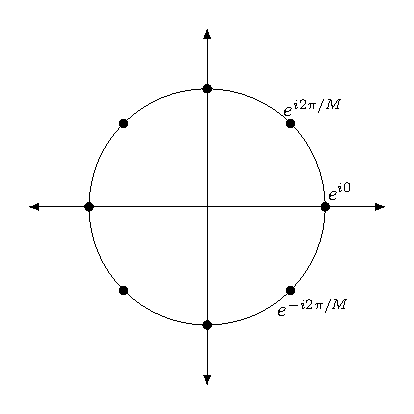
\includegraphics[]{Lectures/Figures/unit_circle_sum.pdf}
    \caption{When looking at $\sum_k e^{ik\delta(j - j')}$, for $k \in \set{-\frac{M}{2} + 1, \ldots, -1, 0, 1, \ldots, \frac{M}{2}} \cdot \frac{2\pi}{L}$, and $\abs{j-j'}=1$, we can view the sum as going over points in the complex unit circle. Above, we have $M = 8$. The sum of the points has its center of mass in the center of the unit circle, i.e. $0$ and so the sum evaluates to zero. For $\abs{j - j'} > 1$, we simply skip points (the sum goes around the circle at ``higher frequency''), but the sum cancells in the same way.}
    \label{fig:unit_circle_sum}
\end{figure}

For $j - j' \neq 0$ in general, we repeat the argument (potentially skipping point as larger $j-j'$ has larger frequency around the circle). This is why we conclude that $\sum_{k}e^{ik\delta(j-j')} = M\delta_{jj'}$.

Let's now convert the action:
\begin{equation}
    \sum_{j=1}^M \phi_j^2 = \frac{1}{M}\sum_j\left(\sum_{j}e^{ik\delta j}\tilde{\phi}_k\right)\left(\sum_{k'}e^{ik'\delta j}\tilde{\phi}_{j'}\right) = \frac{1}{M}\sum_{kk'}\tilde{\phi}_k\tilde{\phi}_{k'}\sum_j e^{ik\delta j}e^{ik'\delta j} = \frac{1}{M}\sum_{kk'}\tilde{\phi}_k\tilde{\phi}_{k'} \sum_{j=1}^M e^{i\delta j (k + k')}
\end{equation}

Applying the same argument as we saw in checking the inverse Fourier transform, we know that $\sum_{j=1}^M e^{i\delta j (k + k')} = M\delta_{k', -k}$ so:
\begin{equation}
    \sum_{j=1}^M \phi_j^2 = \sum_{kk'}\tilde{\phi}_k\tilde{\phi}_{k'}\delta_{k',-k} = \sum_k \tilde{\phi}_k\tilde{\phi}_{-k} = \sum_{k}\abs{\tilde{\phi}_k}^2
\end{equation}
where in the last equality we use the reality condition $(\tilde{\phi}_k)^* = \tilde{\phi}_{-k}$.

The time derivative term works out exactly the same way, just take the dot along for the ride:
\begin{equation}
    \sum_{j=1}^M \dot{\phi_j}^2 = \sum_{k}\abs{\dot{\tilde{\phi}}_k}^2.
\end{equation}

The term that is more subtle (and more interesting) is the interaction term. Let us study this now.

\begin{equation}
    \sum_{j=1}^M (\phi_j - \phi_{j+1})^2 = \frac{1}{M}\sum_j \left(\sum_k \left(e^{ik\delta j}\tilde{\phi}_k - \sum_k e^{ik\delta(j+1)}\tilde{\phi}_{k}\right)\right)^2
\end{equation}
The two terms appearing are almost identical, so we factor out the piece that looks the same:
\begin{equation}
    \sum_{j=1}^M (\phi_j - \phi_{j+1})^2 = \frac{1}{M}\sum_j \left(\sum_k \tilde{\phi}_k e^{ik\delta j}\left(1 - e^{ik\delta}\right)\right)\left(\sum_{k'}\tilde{\phi}_{k'}e^{ik'\delta k}(1 - e^{ik'\delta})\right)
\end{equation}
Now doing the trick we've seen twice already, we interchange the order of the summations and take the $j$ sum first:
\begin{equation}
    \sum_{j=1}^M (\phi_j - \phi_{j+1})^2 = \frac{1}{M}\sum_{kk'}\tilde{\phi}_k \tilde{\phi}_{k'}(1 - e^{ik\delta})(1-e^{ik'\delta})\sum_j e^{i\delta j(k+k')} = \frac{1}{M}\sum_{kk'}\tilde{\phi}_k \tilde{\phi}_{k'}(1 - e^{ik\delta})(1-e^{ik'\delta}) M\delta_{k',-k}
\end{equation}
We are then left with:
\begin{equation}
    \sum_{j=1}^M (\phi_j - \phi_{j+1})^2 = \sum_{k}\tilde{\phi}_k\tilde{\phi}_{-k}(1 - e^{ik\delta})(1-e^{-ik\delta}) = \sum_{k}\abs{\tilde{\phi}_k}^2 (2 - (e^{ik\delta} + e^{-ik\delta})) = 2\sum_k \abs{\tilde{\phi}_k}^2(1-\cos(k \delta))
\end{equation}
where the last equality follows via Euler's formula. We have thus successfully obtained the action $S$ in the $k$-basis. The modes are now not labelled by sites, but by the wavevector (number as we are in 1-D) $k$. 

Question: How could we have guessed that this was a good choice of basis? One intuition is that the action (in the position basis) was translation invariant. When we have a translation invariant problem, momentum is conserved and thus the momentum basis is convenient to work in.

Since we now have diagonalized the action - we have $M$ decoupled QSHOs labelled by $k$; the eigenstates and spectrum easily follow. The eigenstates are:
\begin{equation}
    \ket{\set{n_k}} = \ket{n_{(-\frac{M}{2} + 1)\frac{2\pi}{L}}, \ldots, n_{-\frac{2\pi}{L}}, n_0, n_{\frac{2\pi}{L}}, \ldots, n_{\frac{M}{2}\frac{2\pi}{L}}}
\end{equation}
The energy is simply the sum of the energy of each of the modes:
\begin{equation}
    \hat{H}\ket{\set{n_k}} = E_{\set{n_k}}\ket{\set{n_k}} = \sum_k E_{n_k}\ket{\set{n_k}}
\end{equation}
where:
\begin{equation}
    E_{n_k} = (n_k + \frac{1}{2})\sqrt{\omega_0^2 + 2\frac{c^2}{\delta^2}(1-\cos(\delta k))}
\end{equation}
which is obtained by looking at the action in Eq. \eqref{eq:actionmomentumspace}, and taking the square root of the terms multiplying $\frac{1}{2}\abs{\tilde{\phi}_k}^2$. 

We have thus solved our first nontrivial quantum many-body problem! Although simply, this already has applications in nature; this simple model describes phonons in a crystal, and can be used to predict the heat capacity of a crystal. Note that in a crystal, the spacing $\delta$ is finite (the lattice/atomic spacing). However, what we will do now is take the continuum limit.

\subsection{Continuum Limit: QM to QFT}
What we really did above is solve a quantum-mechanics problem; we now take $\delta \to 0$ and go from QM to QFT. Let's see what happens to the $\frac{c^2}{\delta^2}(1-\cos(\delta k))$ term in this limit. Taylor expanding the cosine, we have:
\begin{equation}
    \lim_{\delta \to 0 }\frac{c^2}{\delta^2}(1 - \cos(\delta k)) = \lim_{\delta \to 0}\frac{c^2}{\delta^2}\left(1 - \left(1 - \frac{(\delta k)^2}{2}\right)\right) = \frac{1}{2}c^2k^2
\end{equation}
Thus the action becomes:
\begin{equation}
    S = \sum_k \int dt \frac{1}{2}\abs{\dot{\tilde{\phi}}_k^2} - \frac{1}{2}(\omega_0^2 + c^2k^2)\abs{\tilde{\phi}_k}^2
\end{equation}
and the spectrum becomes:
\begin{equation}
    E_{n_k} = (n_k + \frac{1}{2})\sqrt{\omega_0^2 + c^2k^2}
\end{equation}
You will explore this a little more in the first problem set.

Let us see what happens in position space in the continuum limit! Recall the action in position space:
\begin{equation}
    S = \sum_{j=1}^M \int dt \frac{1}{2}\dot{\phi}_j^2 - \frac{1}{2}\omega_0^2\phi_j - \frac{1}{2}\frac{c^2}{\delta^2}\left(\phi_j - \phi_{j+1}\right)^2
\end{equation}
Then noting that, $\phi_j = \phi(x = j\delta)$ in the continuum limit the interaction term becomes:
\begin{equation}
    \lim_{\delta \to 0} \left(\frac{\phi(j\delta + \delta) - \phi(j\delta)}{\delta}\right)^2 = (\partial_{x=\delta j} \phi)^2
\end{equation}
where we recognize the definition of the derivative. In addition, the sum over lattice sites becomes an integral over position space, so the action becomes:
\begin{equation}
    S = \int dt \int dx \frac{1}{2}(\partial_t \phi(t, x))^2 - \frac{1}{2}c^2(\partial_x \phi(t, x))^2 - \frac{1}{2}\omega_0^2(\phi(t, x))^2
\end{equation}
where we can (loosely) recognize the wavevector $k$ becoming $\partial_x$ in position space. Now, let's obtain the classical equation of motion for this system:
\begin{equation}
    0 = \delta S = \int dtdx \dot{\phi}\dot{\delta \phi} - c^2 \partial_x \phi \partial_x \delta \phi - \omega_0^2 \phi \delta \phi
\end{equation}
Like last time, we wish to factor out $\delta \phi$, as we can then conclude that whatever it multiples must be zero. We integrate by parts, and we choose the variation to be zero at spatial/temporal infinity so that we may throw away the boundary term (we don't \emph{have} to impose this - not doing so would give us an extra condition, but for now we don't care about the boundaries). We are left with:
\begin{equation}
    0 = \int dt dx \delta \phi(-\partial_t^2\phi + c^2\partial_x^2 \phi - \omega_0^2 \phi)
\end{equation}
and since this must be true for all choices of variations $\delta \phi(t, x)$, we obtain:
\begin{equation}
    \boxed{(\partial_t^2 - c^2\partial_x^2 + \omega_0^2)\phi(t, x) = 0}
\end{equation}
which is the classical equation of motion for this field, known as the \emph{Klein-Gordon equation}. The first two terms we recognize as those appearing in the standard wave equation, with solutions $f(x \pm ct)$. The $\omega_0^2$ is an addition to the wave equation, which tells us that disturbances propagate at speed $< c$. Although the dynamics are a little more complex than the wave equation, it is still a linear PDE and can be solved.

This equation is accidentally relativistic (it is Lorentz covariant, as we shall soon see), without trying. Interestingly, $c$ may not be the speed of light in materials, yet such systems have a sort of Lorentz symmetry.

Note that even with interactions, this QFT is still called free scalar field theory, as the action is quadratic in the field. We will also in the future look at (non-linear) interactions, which will be more difficult and lead to further phenomenology.

\subsection{Lorentz Invariance}
Some systems have relativistic symmetry, in which case we should use it; it is also just a great example of how we can use symmetries to constrain and understand QFTs. Finally, it is a symmetry of nature, so we should care about it, as humans, not just as physicists\footnote{Luca: I try to tell this to my friends, but it doesn't really work...}. Symmetries are described by groups, and then we can do things like classifying particles by representations of groups (e.g. spin-1/2 particles described by representations of the Lorentz group).

Historically, Maxwell's equations were the first hint that the laws of nature are \emph{not} invariant under Galilean boosts:
\begin{equation}
    \v{x} \to \v{x} + \delta\v{v}t, \quad t \to t
\end{equation}
(where time is left invariant) but rather invariant under Lorentz boosts:
\begin{equation}\label{eq:infinitesimalLorentz}
    \v{x} \to \v{x} + \delta\v{v}t, \quad t \to t + \frac{\delta\v{v} \cdot \v{x}}{c^2}
\end{equation}
where we note that time is also transformed. At low velocities $\abs{\v{v}} \ll c$ this effect is small so we may be able to neglect it, but (e.g.) in electromagnetism or in relativistic systems it becomes highly relevant.

From now on, we choose units such that $c = 1$. 

Note that the transformations appearing in Eq. \eqref{eq:infinitesimalLorentz} are the infinitesimal form, but this is all we really need; from these we can easily find the finite versions.

How can we understand Lorentz transformations? They are those that leave \emph{spacetime} distance between pairs invariant:
\begin{equation}
    \abs{\v{x}}^2 - t^2 \to (\v{x} + \delta\v{v}t)^2 - (t + \delta\v{v} \cdot \v{x})^2 = \abs{\v{x}}^2 - t^2 + 2\v{x} \cdot \delta \v{v}t - 2t\v{x}\cdot \delta \v{v} = \abs{\v{x}}^2 - t^2
\end{equation}
where we neglect terms $O((\delta \v{v})^2)$. 

\begin{figure}[htbp]
    \centering
    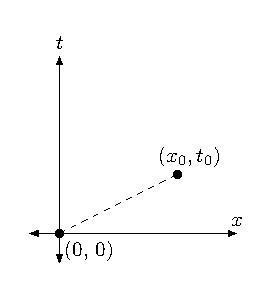
\includegraphics[]{Lectures/Figures/spacetime_interval.pdf}
    \caption{Lorenz transformations leave the \emph{spacetime} distance $\abs{\v{x}}^2 - t^2$ between two spacetime points invariant, here $x_0^2 - t_0^2$.}
    \label{eq:spacetime_interval}
\end{figure}

We here consider a more compact notation in the form of 4-vectors, where we group the 3 spatial and 1 temporal (3+1) coordinates into a single vector:
\begin{equation}
    x^\mu = (t, x^1, x^2, x^3)
\end{equation}
where we can then write the spacetime distance as:
\begin{equation}
    -t^2 + \v{x}^2 = \m{t \\ x_1 \\ x_2 \\ x_3}^T \m{-1 & 0 & 0 & 0 \\ 0 & 1 & 0 & 0 \\ 0 & 0 & 1 & 0 \\ 0 & 0 & 0 & 1}\m{t \\ x_1 \\ x_2 \\ x_3}
\end{equation}
the $4 \times 4$ matrix appearing above is the Minkowski metric $\eta_{\mu\nu} = \text{diag}(-1, 1, 1, 1)$, and we can write the spacetime interval as:
\begin{equation}
    -t^2 + \abs{\v{x}}^2 = x^\mu \eta_{\mu \nu} x^\nu = x^2
\end{equation}
where $\mu, \nu = 0, 1, \ldots, d$ where $x^0 = t$ and $d$ is the spatial dimension, $3$ in this case. This is the correct choice of the metric signature, according to Luca, though it was met with murmurs of mild controversy from the crowd.

\subsection{Classifying all Lorentz Transformations}
Let us try to find \emph{all} Lorentz transformations, i.e. linear transformations:
\begin{equation}
    x^\mu \to \Lambda^{\mu}_\nu x^\nu = x^{,\mu}
\end{equation}
that leave the spacetime interval invariant:
\begin{equation}
    x^2 \equiv x^\mu \eta_{\mu\nu} x^\nu \to \eta_{\mu\nu}x^{'\mu}x^{'\nu} = \eta_{\mu\nu}\Lambda^\mu_\alpha \Lambda^\nu_\beta x^\alpha x^\beta
\end{equation}
This yields the condition:
\begin{equation}
    \eta_{\mu\nu} \Lambda^\mu_\alpha \Lambda^\nu_\beta = \eta_{\alpha\beta}
\end{equation}
i.e. the $\Lambda$ matrices leave the Minkowski metric invariant.

Notice that these include spatial rotations, which rotates space and leaves time invariant! These satisfy $t \to t$ and $\abs{\v{x}}^2 \to \abs{\v{x}}^2$ (rotations leave spatial distances invariant). So, one subclass of Lorentz transformations are
\begin{equation}
    \Lambda = \m{1 & 0 & 0 & 0 \\ 0 & & & \\ 0 & & R & \\ 0 & & &}
\end{equation}
Where $R$ are the $3 \times 3$ rotation matrices satisfying$R^T \cdot R = \II$.

Note that Lorentz transformations form a group; let us check that they satisfy the group axioms. (1) If $\Lambda_1, \Lambda_2 \in G$, then:
\begin{equation}
    (\Lambda_1 \Lambda_2)^T \eta (\Lambda_1 \Lambda_2) = \Lambda_2^T (\Lambda_1^T \eta \Lambda_1) \Lambda_2 = \Lambda_2^T \eta \Lambda_2 = \eta
\end{equation}
so $\Lambda_1\Lambda_2 \in G$. (2) The $\Lambda$s are just matrices, so clearly their multiplication is associative:
\begin{equation}
    \Lambda_1(\Lambda_2\Lambda_3) = (\Lambda_1\Lambda_2)\Lambda_3.
\end{equation}
(3) There exists the identity element $\mathbb{I}$; this is just $\Lambda = \text{diag}(1, 1, 1, 1)$ which maps $x^\mu \to x^\mu$. Finally (4) There exists an inverse $\Lambda^{-1} \in G$ such that $\Lambda^{-1}\Lambda = \mathbb{I}$. Intuitively this is true, e.g. for rotations we just rotate in the opposite direction and that is the inverse transformation. We will examine the condition more closely next class. 
